\section{Operators}\label{sec:operators}
As described in section~\ref{sec:genetics}, genetic operators are used to create
new individuals.
This section presents crossover and mutation genetic operators
that are used for the individual representation from section~\ref{sec:coding}.

\subsection{Crossover}\label{subsec:crossover}

Novel crossover approach proposed in this thesis
creates a new individual by weighted vector addition of the parent's stochastic vectors followed by a normalization back to the stochastic vector.
Using notation from section~\ref{sec:coding}, that is
$PS_{rk}$ for painting sequence random key vector,
$SO_{rk}$ for slicing order random key vector and
$OR_{prob}$ for orientation probabilities matrix,
we can define crossover for two parents $A$, $B$ and offspring $C$ as

\begin{equation}
    \|w_A A_{PS_{rk}} + w_B B_{PS_{rk}}\| = C_{PS_{rk}}\,,
    \label{eq:crossover-psrk}
\end{equation}

\begin{equation}
    \|w_A A_{SO_{rk}} + w_B B_{SO_{rk}}\| = C_{SO_{rk}}\,,
    \label{eq:crossover-sork}
\end{equation}

\begin{equation}
    \|(w_A A_{OR_{prob}i:} + w_B B_{OR_{prob}i:})P\| = C_{OR_{prob}i:}\,,
    \label{eq:crossover-orprob}
\end{equation}

where $\|\cdot\|$ is normalization to the stochastic vector, $+$ is vector addition, $w_A, w_B \in \real$ are weights,
$P \in \real^{N-1}$ is orientation penalization vector with $N$ being instance size, notation $X_{i:}$ means $i$-th row of a matrix $X$
and multiplying a vector by a scalar multiplies each element of the vector by that scalar.

Example of crossover for painting sequence random key and slicing order random key, eq.~\ref{eq:crossover-psrk} and~\ref{eq:crossover-sork},
is in figure~\ref{fig:crossover-random-keys}.
An example of crossover for orientation probabilities, eq.~\ref{eq:crossover-orprob}, is in figure~\ref{fig:crossover-orientation-probabilities}.

The crossover implementation described above has multiple parts – vector sum, weights, orientation penalization and normalization.
Following are arguments for incorporating each of those parts into a crossover.

\subsubsection*{Vector sum}

\subsubsection*{Weights}

\subsubsection*{Orientation penalization}

\subsubsection*{Normalization}

%This implementation of crossover differs from others in a way that there is no copying parts of the chromosome from each parent.
%For example, one-point-crossover~\cite{hollandAdaptationNaturalArtificial1975} that produces an offspring’s chromosome by copying
%first half of the first parent’s chromosome followed by the second’s parent second half of the chromosome.

\begin{figure}[htp]
    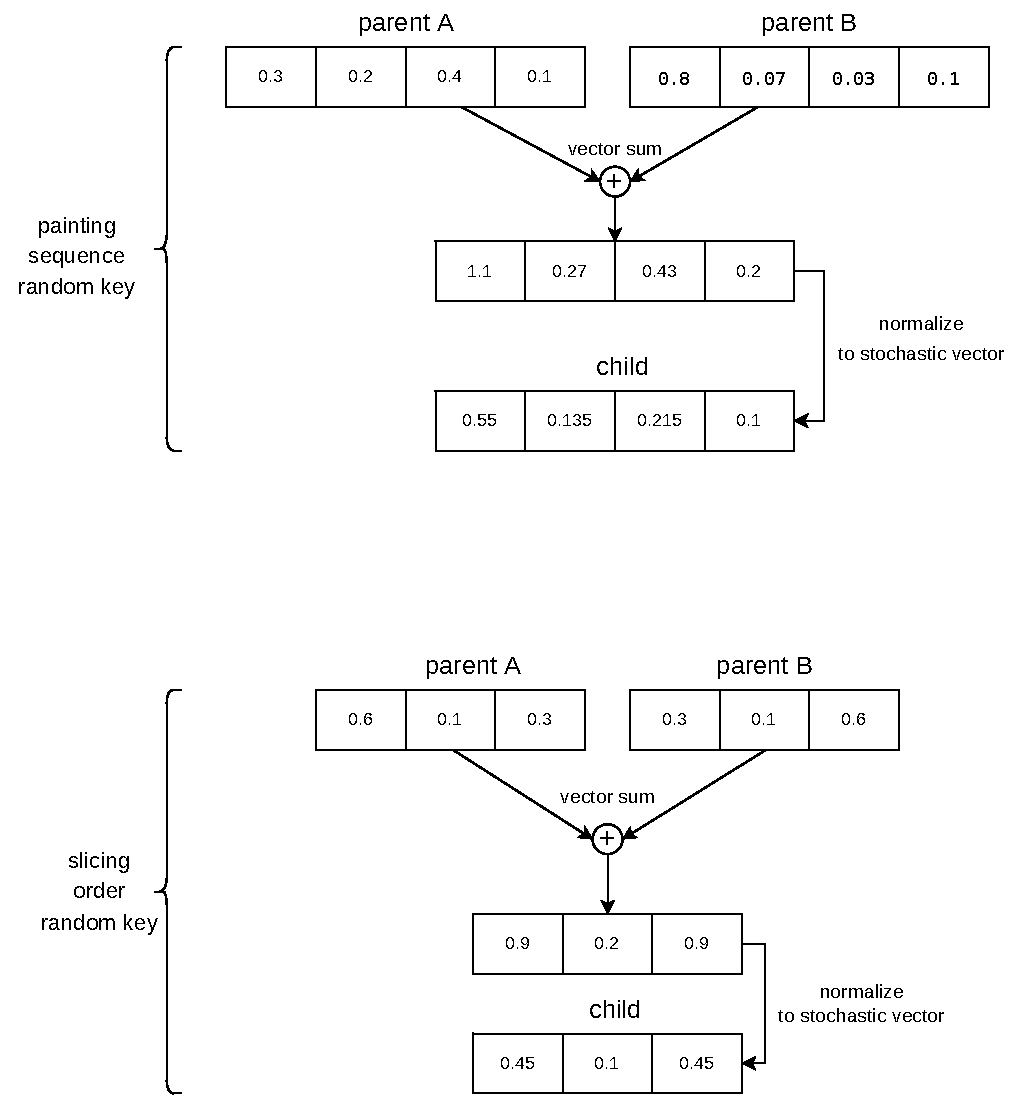
\includegraphics[width=1.0\textwidth, left]{crossover_random_keys}\caption{
        Crossover example for painting sequence and slicing order random keys.
        The procedure is the same for both – sum weighted parent vectors and then normalize to stochastic vector.
    }
    \label{fig:crossover-random-keys}
\end{figure}

\begin{figure}[htp]
    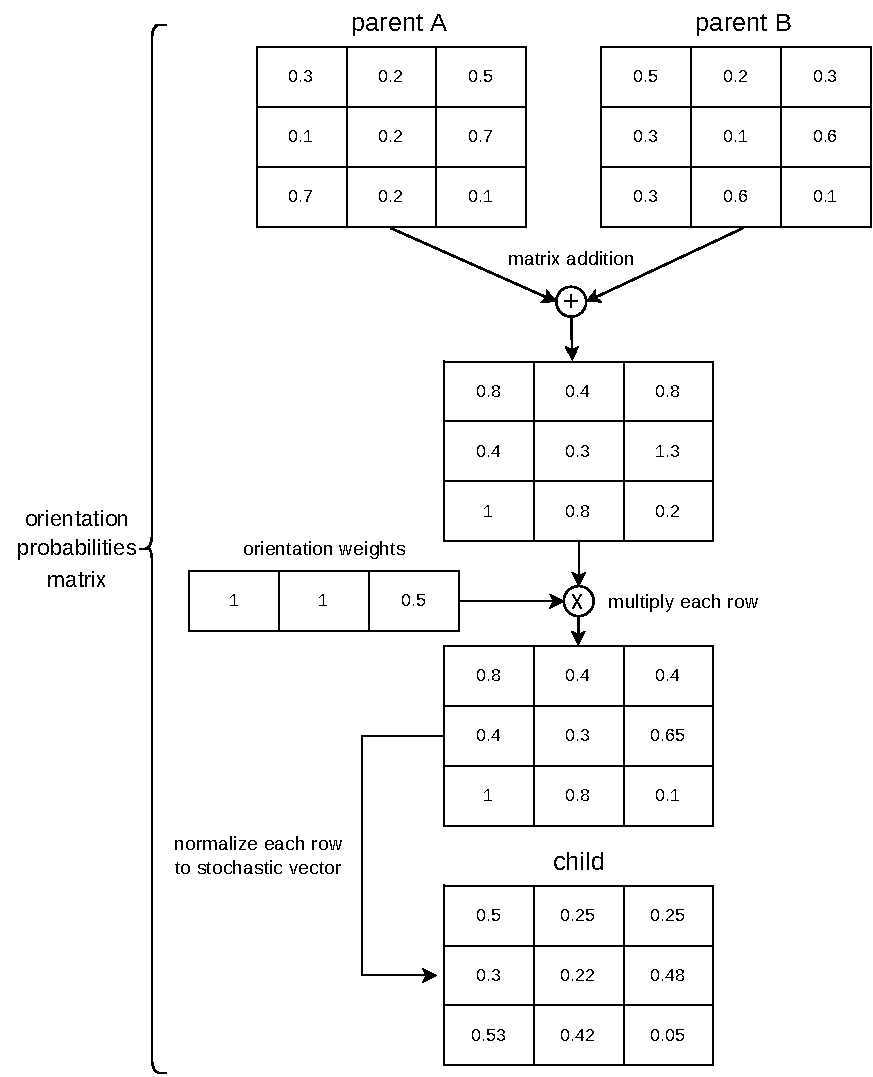
\includegraphics[width=0.85\textwidth, left]{crossover_orientation_probabilities}\caption{
        Crossover example for orientation probabilities. The procedure is first to sum weighted parent matrices,
        then multiply the matrix with orientation penalization vector and normalize each row to a stochastic vector.}
    \label{fig:crossover-orientation-probabilities}
\end{figure}

\subsection{Mutation}\label{subsec:mutation}
